\documentclass[10pt,pdf,utf8,russian,aspectratio=169]{beamer}
\usepackage[T2A]{fontenc}
\usetheme{Singapore}
\usepackage{setspace}
\usepackage{amsmath}
\usepackage{pgfplots}
\usepackage[utf8]{inputenc}
\usepackage{tikz-cd}
\usepackage[all, 2cell]{xy}
\usepackage{amssymb}
\usepackage{verba tim}
\usepackage[all]{xy}
\usepackage{tikz}
\usepackage{bussproofs}
\usepackage{dsfont}
\usepackage{mathabx}
\usepackage{animate}
\usetikzlibrary{graphs}
\usetikzlibrary{arrows}
\usepackage{hyperref}
\usepackage[english,russian]{babel}
\usepackage{listings}
\usepackage{color}
\usepackage{tikz}
\usepackage{listings}
\pgfplotsset{compat=1.16}
\newtheorem{defin}{Definition}
\newtheorem{theor}{Theorem}
\newtheorem{prop}{Proposition}
\title{Functional programming, Seminar No. 2}
\author{Danya Rogozin \\ Lomonosov Moscow State University, \\ Serokell O\"{U}}
\date{Higher School of Economics \\ Faculty of Computer Science}
\begin{document}
\lstset{
  frame=none,
  xleftmargin=2pt,
  stepnumber=1,
  numbers=left,
  numbersep=5pt,
  numberstyle=\ttfamily\tiny\color[gray]{0.3},
  belowcaptionskip=\bigskipamount,
  captionpos=b,
  escapeinside={*'}{'*},
  language=haskell,
  tabsize=2,
  emphstyle={\bf},
  commentstyle=\it,
  stringstyle=\mdseries\rmfamily,
  showspaces=false,
  keywordstyle=\bfseries\rmfamily,
  columns=flexible,
  basicstyle=\small\sffamily,
  showstringspaces=false,
  morecomment=[l]\%,
}
\maketitle

\begin{frame}[fragile]
  \frametitle{Bindings}

  The equality sign in Haskall denotes binding:

    \begin{lstlisting}[language=Haskell]
      fortyTwo = 42
      coolString = "coolString"
    \end{lstlisting}

\vspace{\baselineskip}

Local binding with the \verb"let"-keyword:
  \begin{lstlisting}[language=Haskell]
    fortyTwo = let number = 43 in number - 1
  \end{lstlisting}
\end{frame}

\begin{frame}[fragile]
  \frametitle{Function definitions}

  Functions are also defined as bindings:

  \begin{lstlisting}[language=Haskell]
    add x y = x + y
    userName name = "Username: " ++ name
    id x = x
  \end{lstlisting}

  \vspace{\baselineskip}

  The same functions defined via lambda:
  \begin{lstlisting}[language=Haskell]
    add = \x y -> x + y
    userName = \name -> "Username: " ++ name
    id = \x -> x
  \end{lstlisting}
\end{frame}

\begin{frame}[fragile]
  \frametitle{Function application}

  As in lambda calculus, function application is right associative by default

  \begin{lstlisting}[language=Haskell]
    {-
    foo x y z = f x y z = ((f x) y) z
    -}
  \end{lstlisting}

\vspace{\baselineskip}

  One may use the dollar infix operator in order to avoid brackets overuse. For example, the following functions have exactly the same behaviour:

  \begin{lstlisting}[language=Haskell]
    function f x y z = f ((x y) z)
    function1 f x y z = f $ x y $ z
  \end{lstlisting}
\end{frame}

\begin{frame}[fragile]
  \frametitle{Prefix and infix notation}
  Any operator or function might be called in prefix and infix:

  \begin{center}
  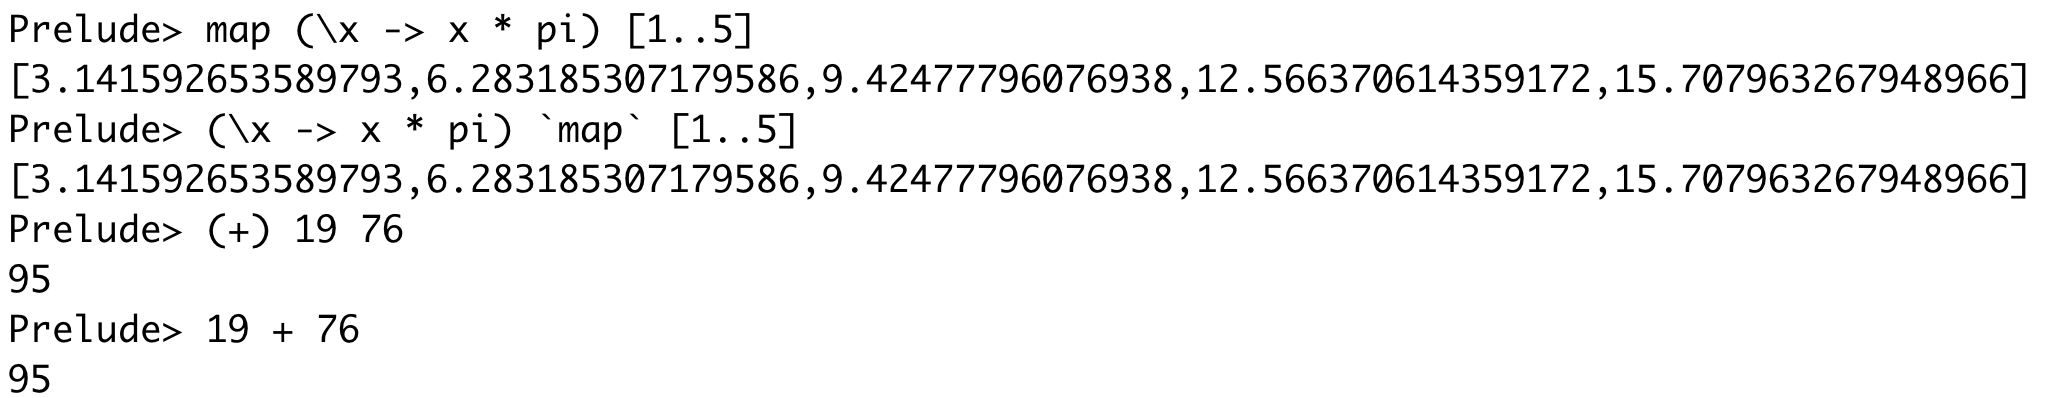
\includegraphics[scale=0.41]{Pics/InfixPrefix.png}
  \end{center}

  \vspace{\baselineskip}

  One may declare an operator defining its priority and associativity explicitly. Here's an example:

\begin{lstlisting}[language=Haskell]
(&&) :: Bool -> Bool -> Bool
infixr 3 &&
\end{lstlisting}
\end{frame}

\begin{frame}[fragile]
  \frametitle{Currying and partial application}

Let us recall the function \verb"add" once more:

\begin{lstlisting}[language=Haskell]
  add x y = x + y
\end{lstlisting}

Here is an example of a partial application in the following GHCi session

\vspace{\baselineskip}

\begin{lstlisting}[language=Haskell]
add x y = x + y
addFive = add 5
twentyEight = addFive 23
  -- 28
\end{lstlisting}

Partial application is well-defined since all many-argument functions in Haskell are curried by default.

\end{frame}

\begin{frame}[fragile]
  \frametitle{Immutability and laziness}

In Haskell, values are immutable. The GHCi example:

\begin{center}
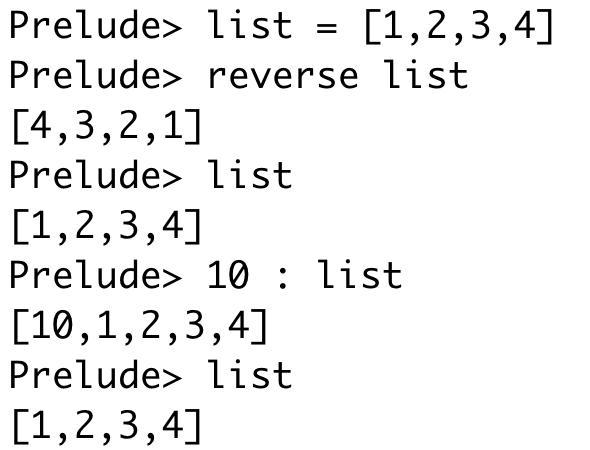
\includegraphics[scale=0.41]{Pics/Imm.png}
\end{center}
\end{frame}

\begin{frame}[fragile]
  \frametitle{Recursion}

  The straightforward recursion:
  \begin{lstlisting}[language=Haskell]
    factorial n = if n == 0 then 1 else n * factorial (n - 1)
  \end{lstlisting}

  \vspace{\baselineskip}

  The factorial function implemented via so-called tail recursion:
  \begin{lstlisting}[language=Haskell]
    tailFactorial n = helper 1 n
      where
      helper acc x =
        if x > 1
        then then helper (acc * x) (x - 1)
        else acc
  \end{lstlisting}
\end{frame}

\begin{frame}[fragile]
  \frametitle{Guards}

  Let us take a look at the factorial implementation via guards:

  \begin{lstlisting}[language=Haskell]
    tailFactorial n = helper 1 n
      where
      helper acc x | x > 1 = helper (acc * x) (x - 1)
                   | otherwise acc
  \end{lstlisting}
\end{frame}

\begin{frame}[fragile]
  \frametitle{Basic datatypes}
  The basic datatypes are:
  \begin{itemize}
    \item \verb"Bool": Boolean values
    \item \verb"Int": Bounded integer datatype
    \item \verb"Integer": Unbounded integer datatype
    \item \verb"Char": Unicode characters
    \item \verb"()": Unit value datatype
    \item If \verb"a" and \verb"b" are types, then \verb"a -> b" is a type
    \item If \verb"a" and \verb"b" are types, then \verb"(a,b)" is a type
    \item If \verb"a" is a type, then \verb"[a]" is a type
  \end{itemize}

  A type declaration has the following form:

  \begin{lstlisting}[language=Haskell]
    term :: type
  \end{lstlisting}
\end{frame}

\begin{frame}
  \frametitle{Datatypes and constructors}
 Let us recall the list of basic data types above and associative constructors with them. A constructor is a term that allows one to obtain a value of the desired type.
\begin{center}
\begin{tabular}{ |c|c| }
\hline
\verb"Bool": Boolean values & \verb"True" and \verb"False" \\
\verb"\verb"Int": Bounded integer datatype" & Integers from $-2^{29}$ to $2^{29} - 1$ \\
\verb"Integer": Unbounded integer datatype & The set of integers \\
\verb"Char": & Characters \verb"'0'", ..., \verb"'9'", \verb"'a'", ..., \verb"'z'", etc \\
\verb"()": Unit value datatype: & Just \verb"()" \\
\verb"a -> b": & $\lambda x \rightarrow m$ \\
\verb"(a,b)": & if \verb"x :: a" and \verb"y :: b", then \verb"(x, y) :: (a,b)" \\
\verb"[a]", the type of list of elements from \verb"a": & the empty list \verb"[]" \\
\verb"[a]", the type of list of elements from \verb"a": & if \verb"x :: a" and \verb"xs :: [a]", then \verb"x : xs :: [a]" \\
\hline
\end{tabular}
\end{center}
\end{frame}

\begin{frame}
  \frametitle{Types in GHCi}

  The command \verb":t" yields a type of a required expression:

  \begin{center}
  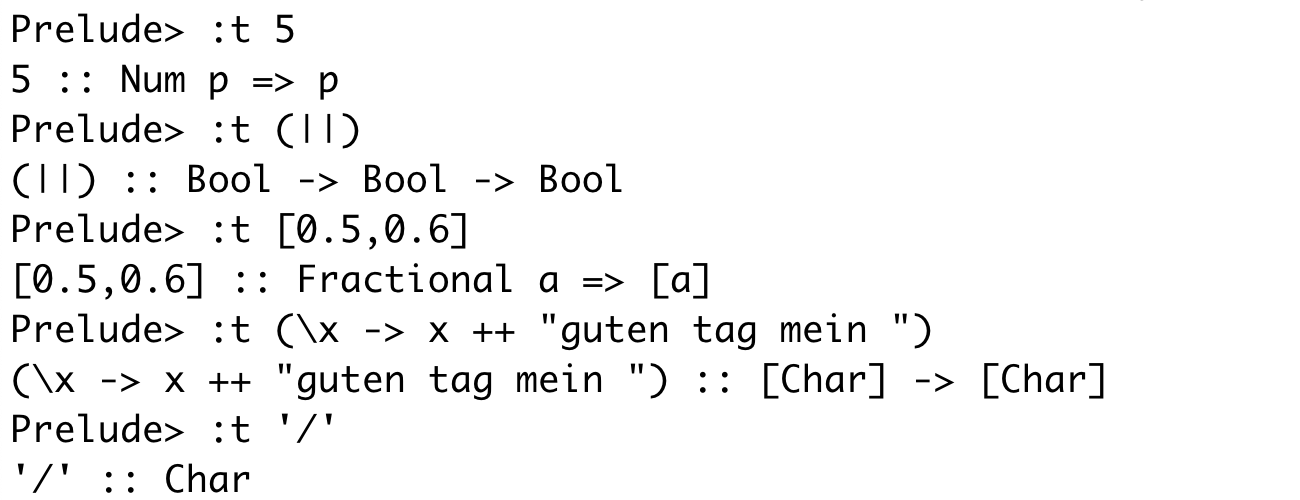
\includegraphics[scale=0.5]{Pics/TypesScreen.png}
  \end{center}

\end{frame}

\begin{frame}[fragile]
  \frametitle{Function declaration with datatypes}

  Let us recall the examples of function declarations:

    \begin{lstlisting}[language=Haskell]
      add x y = x + y
      userName name = "Username: " ++ name
      id x = x
    \end{lstlisting}

    \vspace{\baselineskip}

    One may annotate these functions with types as follows:

    \begin{lstlisting}[language=Haskell]
      add :: Int -> Int -> Int
      add x y = x + y

      userName :: String -> String
      userName name = "Username: " ++ name

      id :: Char -> Char
      id x = x
    \end{lstlisting}

\vspace{\baselineskip}

  Note that such calls as \verb"userName 5" or \verb"id ''hello stewart''" cause type errors.

\end{frame}

\begin{frame}[fragile]
  \frametitle{Lists}

  Let's talk about lists a slightly closely. In Haskell, a list is a homogeneous collection of elements.

  \begin{lstlisting}[language=Haskell]
    empty :: [Int]
    empty = []

    ten :: [Int]
    ten = [10]

    tenEleven :: [Int]
    tenEleven = 11 : ten

    tenElevenTwelve :: [Int]
    tenElevenTwelve = 12 : tenEleven
    -- 12 : (11 : [])
  \end{lstlisting}

\end{frame}

\begin{frame}[fragile]
  \frametitle{Lists. Ranges}

  \begin{lstlisting}[language=Haskell]
  oneToFive :: [Int]
  oneToFive = [1..5]

  oneToSevenOdd :: [Int]
  oneToSevenOdd = [1,3..7]

  nat :: [Int]
  nat [0,1..]

  evens :: [Int]
  evens = [0,2,4..]
  \end{lstlisting}
\end{frame}

\begin{frame}
  \frametitle{Lists. Heads and Tails}
  \begin{minipage}{0.5\textwidth}
    \begin{flushleft}
      \begin{center}
      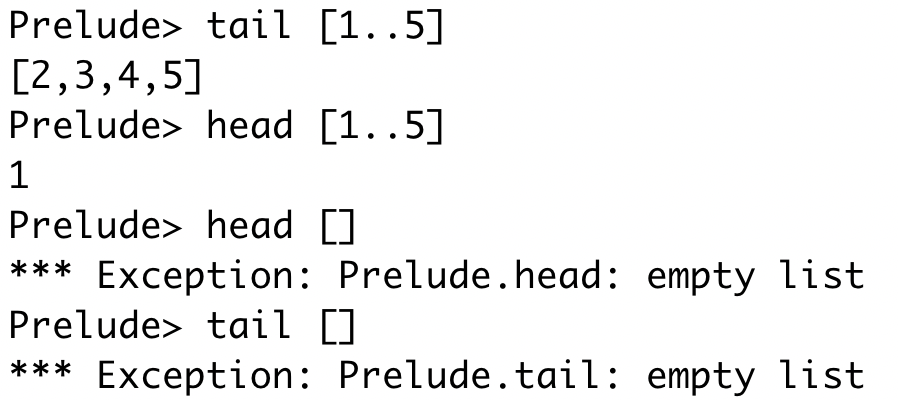
\includegraphics[scale=0.5]{Pics/HeadTail.png}
      \end{center}
    \end{flushleft}
  \end{minipage}\hfill
  \begin{minipage}{0.5\textwidth}
    \begin{flushright}
      \begin{center}
      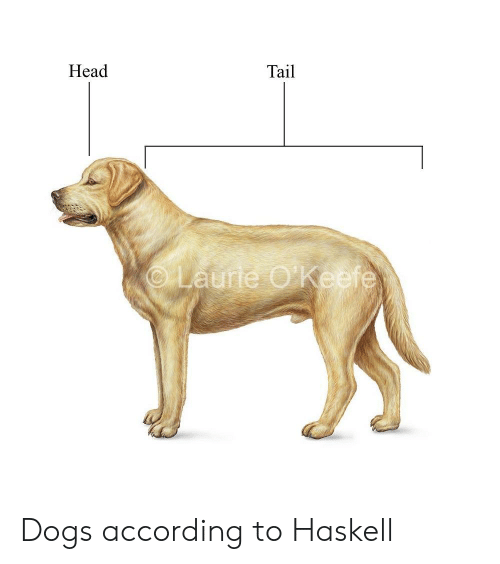
\includegraphics[scale=0.25]{Pics/Doge.png}
      \end{center}
    \end{flushright}
  \end{minipage}

\end{frame}

\begin{frame}
  \frametitle{Other helpful list functions}

  \begin{center}
  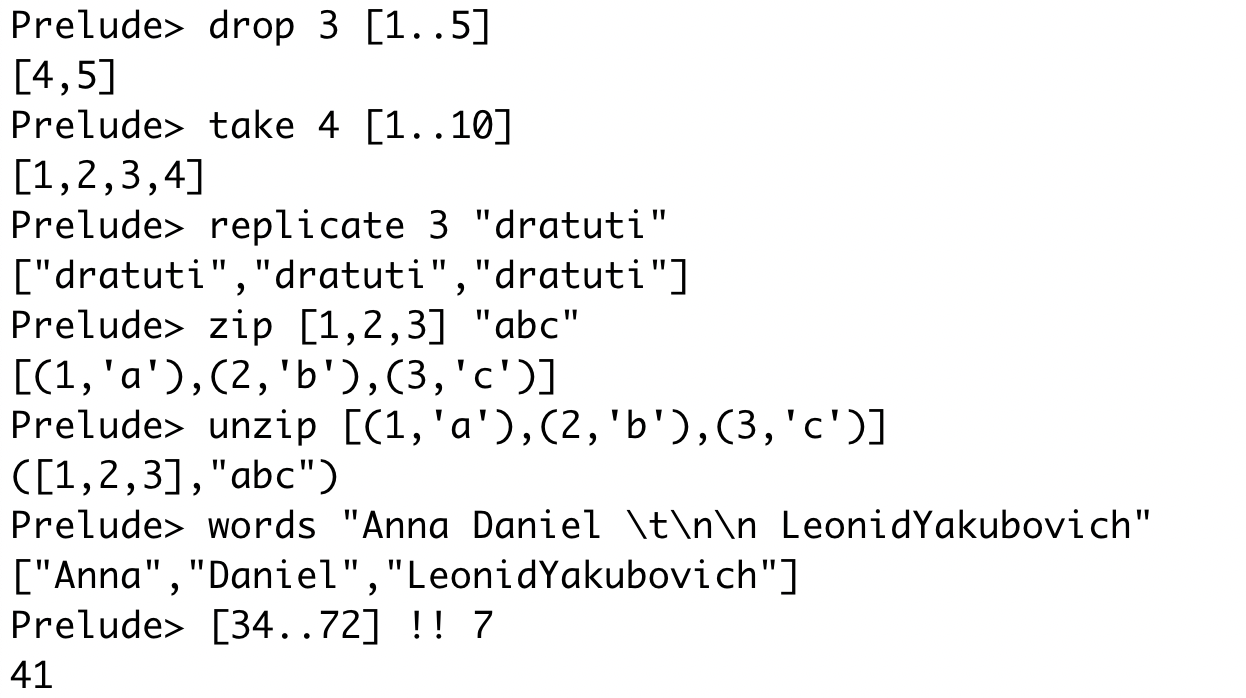
\includegraphics[scale=0.5]{Pics/ListFunctions.png}
  \end{center}

\end{frame}

\begin{frame}
  \frametitle{List compeherension}

  \begin{center}
  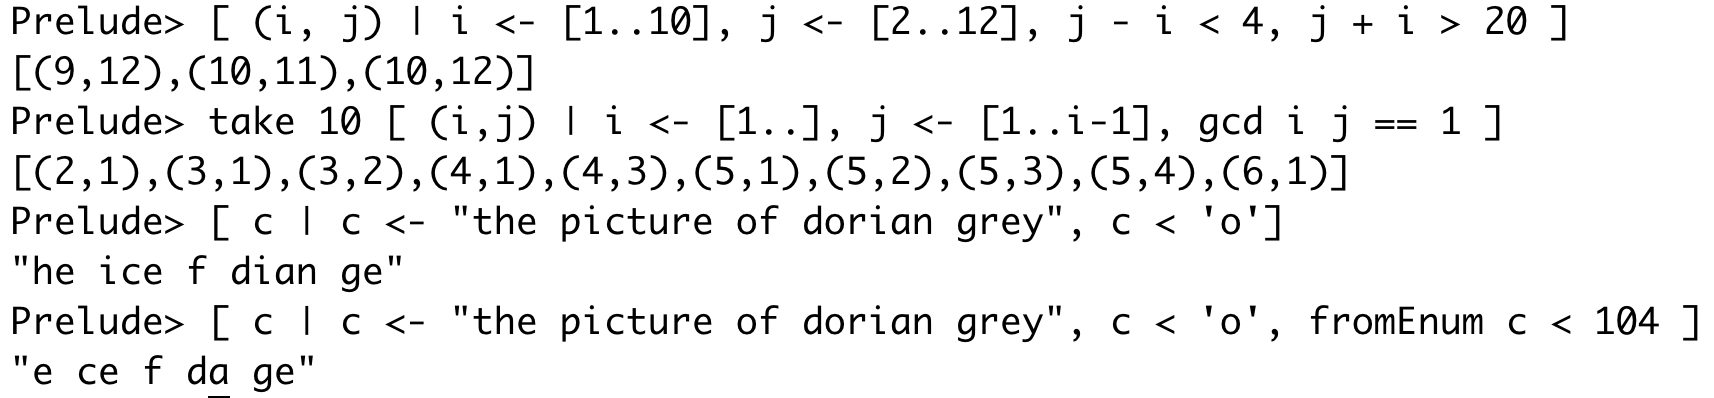
\includegraphics[scale=0.47]{Pics/Compr.png}
  \end{center}
\end{frame}

\begin{frame}[fragile]
  \frametitle{Higher order functions}

  Function is a first-class object and one may pass any function as an argument:

  \begin{lstlisting}[language=Haskell]
  inc, dec :: Int -> Int
  inc x = x + 1
  dec x = x - 1

  changeTwiceBy :: (Int -> Int) -> Int -> Int
  changeTwiceBy operation value = operation (operation value)

  seven :: Int
  seven = changeTwiceBy inc 5

  three :: Int
  three = changeTwiceBy dec 5
  \end{lstlisting}
\end{frame}

\begin{frame}[fragile]
  \frametitle{\verb"Case"-expressions}

\verb"Case"-expressions allows one to perform case analysis within an observed function.

  \begin{lstlisting}[language=Haskell]
getFont :: Int -> String
getFont n =
  case n of
    0 -> "PLAIN"
    1 -> "BOLD"
    2 -> "ITALIC"
    _ -> "UNKNOWN"
  \end{lstlisting}
\end{frame}

\begin{frame}
  \frametitle{Theoretical Flashback. Reduction strategies}

  Here we recall some of relatable definition from lambda calculus:

  \begin{enumerate}
    \item A term $M$ is called \emph{weakly normalisable} (WN), if there exists some halting reduction path that starts from $M$
    \item A term $M$ is called \emph{strongly normalisable} (SN), if any reduction path that starts from $M$ terminates
  \end{enumerate}

  It is clear, that SN implies WN, not vice versa. In other words, there exists a term, that has an infinite reduction path, but it has a finite reduction path.
\end{frame}

\begin{frame}
  \frametitle{Theoretical Flashback. Reduction strategies}

\onslide<1->{
  Let us consider the example of the following ridiculous term: $(\lambda x y. x) (\lambda z. z) ((\lambda x. x x) (\lambda x. x x))$. One may reduce this term in two ways:
}

  \vspace{\baselineskip}
\onslide<2->{
From the one hand:

  $\begin{array}{lll}
  &(\lambda x y. x) (\lambda z. z) ((\lambda x. x x) (\lambda x. x x)) \rightarrow_{\beta} & \\
  &(\lambda y. [x := (\lambda z. z)]) ((\lambda x. x x) (\lambda x. x x)) \rightarrow_{\beta} & \\
  &(\lambda y. \lambda z. z) ((\lambda x. x x) (\lambda x. x x)) \rightarrow_{\beta}& \\
  &(\lambda z. z) [y := (\lambda x. x x) (\lambda x. x x)] \rightarrow_{\beta}& \\
  &\lambda z. z&
  \end{array}$
}
  \vspace{\baselineskip}

\onslide<3->{
  From the other hand:

  $\begin{array}{lll}
  & (\lambda x y. x) (\lambda z. z) ((\lambda x. x x) (\lambda x. x x)) \rightarrow_{\beta} & \\
  & (\lambda x y. x) (\lambda z. z) (x x)(x := [\lambda x. x x]) \rightarrow_{\beta}& \\
  & (\lambda x y. x) (\lambda z. z) ((\lambda x. x x) (\lambda x. x x)) \rightarrow_{\beta} \dots & \\
  & \text{ spasiti pamagiti pajalusta ya tak bolshe ni magu (((((((9(99(}&
  \end{array}$
}
\end{frame}

\begin{frame}
  \frametitle{Theoretical Flashback. Reduction strategies}
  \onslide<1->{
  Let us consider the example above in some other aspects.
  } \onslide<2->{
  \begin{itemize}
    \item In the first case, we have got a sensible result by several reduction steps. On the other hand, we have a loop in the second case.
    } \onslide<3->{
    \item Also, in the first case, we started our reduction from the leftmost innermost redex. When we tried to start our reduction from the right redex $(\lambda x. x x) (\lambda x. x x)$, we have found ourselves in a spot of trouble. Something went wrong.
    } \onslide<4->{
    \item Can we distinguish all possible ways of term reduction?
    }
  \end{itemize}

\onslide<5->{
  In a matter of fact, we need to distinguish all possible ways of application reduction, so far as we have no other options in the remaining cases:

  \begin{enumerate}
    \item If $x$ is a variable, then $x$ is already in normal form
    \item If a term has the form $\lambda x. M$, then we reduce $M$
  \end{enumerate}
  }
\end{frame}

\begin{frame}
  \frametitle{Theoretical Flashback. Reduction strategies}

\onslide<1->{
  Thus, one needs to overview of the possible ways of application reduction. We have two chairs:
} \onslide<2->{
  \begin{enumerate}
    \item $(\lambda x. M) N_1 \dots N_n$: we firtsly reduce $(N_i)_{i \in \{ 1, \dots, n \}}$
    \item $(\lambda x. M) N_1 \dots N_n$: reduce $(\lambda x. M) N_1$ and go further from left to right
  \end{enumerate}
} \onslide<3->{

  The first way is called \emph{applicative order}, the second one is normal one. In the following sense, normal order is better:
} \onslide<4->{
  \begin{theorem}
    Let $M$ be a term such that $M$ has a normal form $M'$, then $M$ might be reduced to $M'$ via normal order
  \end{theorem}
  }
\end{frame}

\begin{frame}
  \frametitle{Theoretical Flashback. Call-by-value and call-by-name}

\begin{itemize}
  \onslide<1->{\item The applicative (normal) order is often called call-by-value (call-by-name)}
  \onslide<2->{\item The most mainstream programming languages you know (Java, Python, Kotlin, etc) have call-by-value semantics}
  \onslide<3->{\item The Haskell reduction has a call-by-value strategy. Informally, such a stragety is called \emph{lazy}. Laziness denotes that Haskell doesn't compute a value if it's not needed at the moment}
  \onslide<4->{\item Call-by-name reduction reduces reducible terms to the bitter end, but it's not always optimal, unfortunately}
\end{itemize}
\end{frame}

\begin{frame}[fragile]
  \frametitle{Haskell reduction}

  Suppose we have such a trivial function:
  \begin{lstlisting}[language=Haskell]
  square :: Int -> Int
  square x = x * x
  \end{lstlisting}

  \vspace{\baselineskip}

\onslide<2->{
  If we call this function on $(1 + 2)$, then we would have the following story:

  $\operatorname{square} \: (1 + 2) = (1 + 2) * (1 + 2) = 3 * (1 + 2) = 3 * 3 = 9$
}
  \vspace{\baselineskip}

\onslide<3->{
  We evalutate $(1 + 2)$ twice, even if we know that $1 + 2 = 3$ a priori.} \onslide<4->{I sincerely hope that you have no doubts about it.} \onslide<5->{The question of optimality is still relevant.
    \begin{center}
    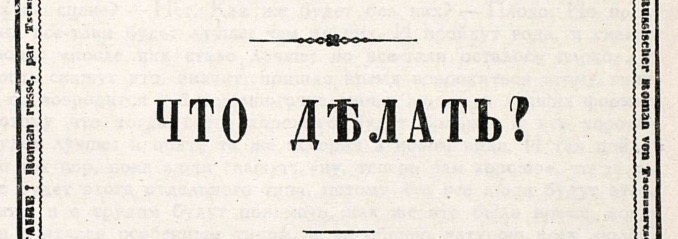
\includegraphics[scale=0.3]{Pics/WhatToDo.jpeg}
    \end{center}
  }
\end{frame}

\begin{frame}[fragile]
  \frametitle{The notion of a weak head normal form}

  In Haskell, reduction evalutates a term to a weak head normal form, where the outermost must be either constructor or lambda. Here are example: WHNFs from the left and non-WHNFs from the right

\begin{minipage}{0.5\textwidth}
  \begin{flushleft}
    \begin{lstlisting}[language=Haskell]
    78

    2 : [1,2]

    'p' : ("ri" ++ "vet")

    [1, 1 + 2, 1 + 3]

    ("hel" ++ "lo", "world")

    \x -> (x + 2) + 2

    \xs -> zip xs [1, 3+2]
    \end{lstlisting}
  \end{flushleft}
\end{minipage}\hfill
\begin{minipage}{0.5\textwidth}
  \begin{flushright}
    \begin{lstlisting}[language=Haskell]
    1 + 665

    (\x -> x ++ "guten tag mein herr ") "Heinrich"

    length [1..145]

    (\f g x -> f (g x)) $ (\x y -> y)
    \end{lstlisting}
  \end{flushright}
\end{minipage}
\end{frame}

\begin{frame}
  \frametitle{Pure functions and side-effects}

  \begin{itemize}
    \onslide<1->{\item A function is called \emph{pure} if it yields the same value for the same argument each time
    \item In other words, a pure function is a function that satisfies Church-Rosser property
    }
    \onslide<2->{\item It means that, such a function has the same behaviour at every point. This principle is also called \emph{referential transparency}
    }
    \onslide<3->{\item A side-effect function is a function that may yield different value passing the same arguments. Mathematically, such a function is not function at all.
    } \onslide<4->{
    \item Haskell functions are (mostly) pure ones, but Haskell isn't confluent as a version of lambda calculus
    }
  \end{itemize}
\end{frame}

\begin{frame}[fragile]
  \frametitle{The failure of confluece}

  Let us consider the following quite simple example. In Haskell one has a function called \verb"seq". According to Hackage, ``The value of \verb"seq a b" is bottom if a is bottom, and otherwise equal to b.'' The listing below demostrates the failure of confluence:

  \begin{lstlisting}[language=Haskell]
  seq :: a -> b -> b
  seq _|_ _ = _|_
  seq _ b   = b

  dno = undefined

  seq dno 14        == dno
  seq (dno . id) 14 == 14
  \end{lstlisting}

\end{frame}

\begin{frame}
  \frametitle{Finally}

\onslide<1->{
  On this seminar, we
  \begin{itemize}
    \item got acquinted with the basic Haskell syntax and basic data types
    \item learnt the underlying aspects of Haskell semantics
    \item discussed pure functions and the example of the confluence failure
  \end{itemize}
}

On the next seminar, we
\begin{itemize}
  \item start to learn polymorphism and its advantages
  \item introduce typeclasses
  \item study the first examples of crucially important examples of type classes
\end{itemize}
\end{frame}

\end{document}
